\chapter{Fortwährender Bot-Support}
Neben den Chatbot-Funktionen, die in dieser Projektarbeit implementiert wurden, war es zudem notwendig, einige weitere Funktionen hinzuzufügen. Neben einer Erweiterung der Einstellungen wurden zudem bestehende Fehlfunktionen behoben, ein Broadcasting-Feature implementiert und eine Hilfsfunktion gebaut.

\section{Anpassung der Befehle}\label{sec:commands}
Telegram empfiehlt den Entwickeln von Bots drei Grundbefehle zu unterstützen, damit der User sich besser zurechtfinden kann und somit die Usability verbessert wird.~\footnote{\url{https://core.telegram.org/bots\#global-commands}}
Diese drei Befehle lauten \texttt{/start}, \texttt{/settings} und \texttt{/help}. Im Zuge dessen wurde der Befehl \texttt{/settings} erweitert und \texttt{/help} implementiert. \texttt{/start} wird beim Starten eines Bots automatisch aufgerufen und ist daher immer Teil des Bots. Beim IWINewsBot wird dann das Abo der Nachrichten gestartet.

\subsection{Broadcasting}
Der IWINewsBot hat mittlerweile über 75 Benutzer und am Ende dieser Projektarbeit gilt es, diese über die neuen Funktionen, die durch die Chatbot-Erweiterung hinzukommen, zu informieren. Dazu wurde ein neuer Telegram-Command namens \texttt{/announce} hinzugefügt. Dieser gibt registrierten Administratoren die Möglichkeit per Telegram eine Nachricht an alle Benutzer des Bots zu schicken, um sie schnell über Updates oder mögliche Fehler zu informieren. \\
Im Bezug auf die neuen Funktionalitäten des Bots wird zu diesem Zwecke ein Telegraph-Blogeintrag verfasst, der die neuen Änderungen mit Beispielen zusammenfasst. So werden sich auch bestehende Benutzer in die neuen Funktionen einfinden. \\
Telegraph\footnote{\url{http://telegra.ph/)}} bietet ohne Login eine Plattform, um schnell einen Blogeintrag zu verfassen. Es generiert dann eine URL, über den der Eintrag öffentlich verfügbar gemacht wird. \\
Telegram bietet für solche Blogeinträge eine Vorschau innerhalb Telegrams, um ihn direkt in der App lesen zu können.

\subsection{Hilfe}
Der \texttt{/help}-Befehl soll eine kurze Übersicht über die Funktionen des Bots bereitstellen. Er listet alle Bot-Commands auf und gibt den Benutzern Anregungen für mögliche Formulierungen, um den Chatbot zu bedienen.

\subsection{Einstellungen}
In der vorherigen Version war es möglich, dass man die Mensapreise über den Befehl \texttt{/settings} und die Abonnements über den Befehl \texttt{/abo} verwalten konnte. Da für die Stundenplan-Funktion Kenntnis über das Semester eines Users benötigt wird, kam diese Einstellungsoption zu den zwei bestehenden hinzu. Um den User nicht mit unnötig vielen Commands zu verwirren und ein einheitliches Einstellungsinterface anzubieten, wurde der \texttt{/settings}-Befehl angepasst, sodass hiermit alle Einstellungen geändert werden können.
Um diese Einstellungen umzusetzen, war es notwendig eine Pseudo-Menüführung anzubieten, die die einzelnen Einstellungsmöglichkeiten öffnet. Dies wurde durch Inline-Buttons ermöglicht. Es können die folgenden Einstellungen vorgenommen werden:
\begin{enumerate}[noitemsep]
    \item Abonnements
    \item Mensapreise
    \item Studiumseinstellung
\end{enumerate}
Die ersten beiden Einstellungen werden mit dem Starten des Bots automatisch gesetzt. So erhält ein neuer User per Default alle Nachrichten (INFB, MKIB, INFM und IWI) und bekommt die Preise für Studierende und Mitarbeiter angezeigt. Die Semester-Einstellungen werden nicht gesetzt.
Diese getroffenen Einstellungen werden dem User bei Aufruf des Commands \texttt{/settings} direkt angezeigt.

\begin{figure}[H]
    \centering
    \caption{/settings-Befehl des IWINewsBot}
      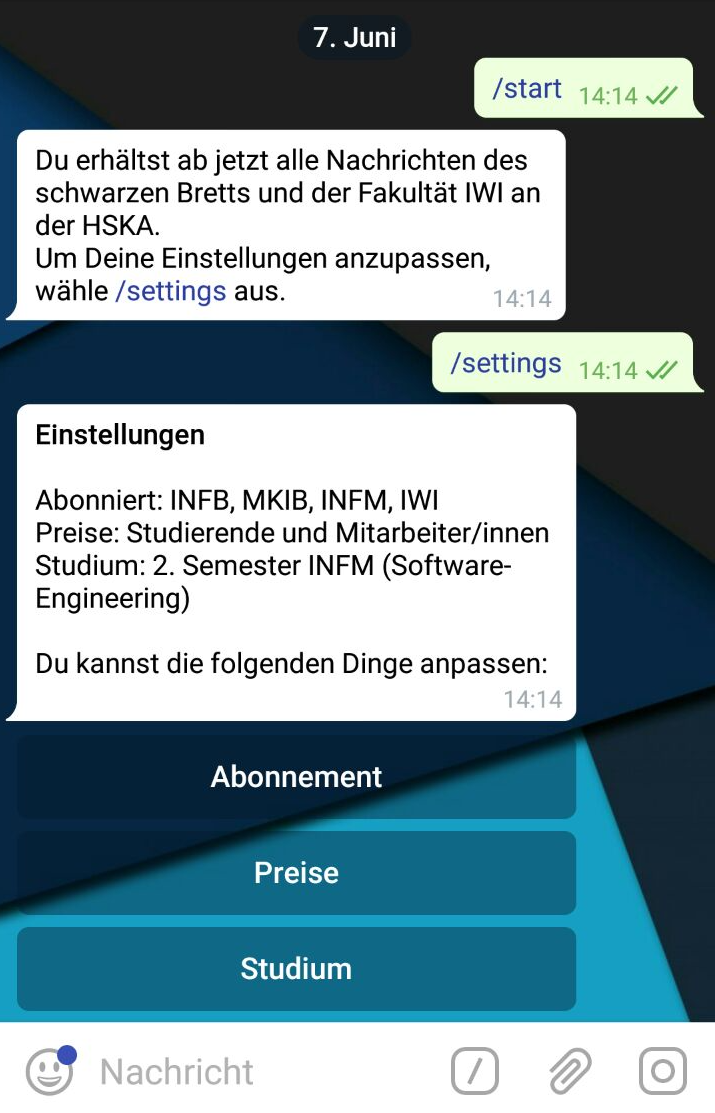
\includegraphics[width=0.4\linewidth]{settings-overview.png}
      \label{img:settings}
    \caption*{Quelle: Eigene Abbildung}
\end{figure}

Die Abonnement-Einstellung an sich hat sich zu der vorherigen Version nicht geändert, hier lässt sich der eingestellte Wert durch Inline-Buttons toggeln und eine Benachrichtung erläutert den eingestellten Wert. Die Mensapreis-Einstellung hingegen hat sich in dieser Version geändert. Hier wurde zuvor über die drei verschiedenen Werte (Studierende / Mitarbeiter / Beides) getoggelt. Dies wird in dieser Version umgangen, indem die einzelnen Optionen selektiert werden können und man mit der Selektion direkt zum Haupt-Screen zurückgelangt. Prinzipiell gibt es für alle Untermenüs die Option, zum Haupt-Screen zurückzugelangen.

\begin{figure}[H]
    \centering
    \caption{Setzen der Mensapreise}
      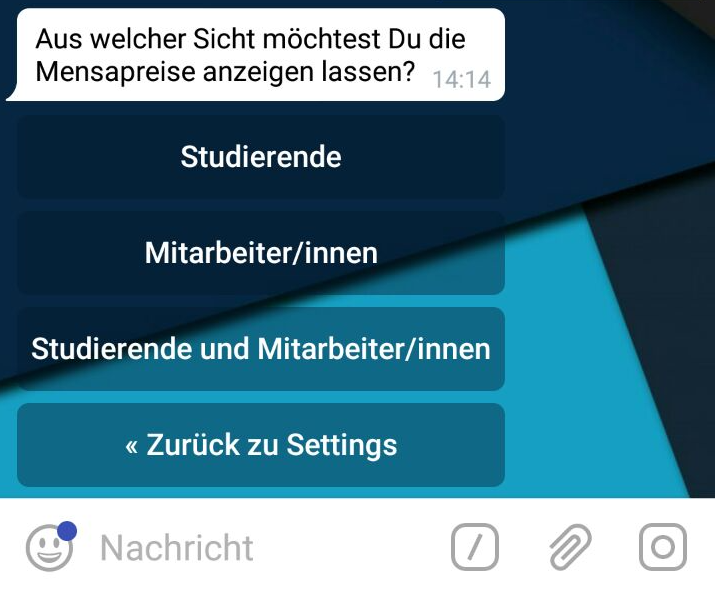
\includegraphics[width=0.4\linewidth]{Mensapreise.png}
      \label{img:mensapreise}
    \caption*{Quelle: Eigene Abbildung}
\end{figure}

Die neueste Einstellung ist die Studiumseinstellung, bei der ein User sein aktuelles Semester wählen kann, um seinen Stundenplan abzufragen. Hierbei wird der User durch ein Menü geführt, bei dem er zuerst sein Studium auswählt, dann seine Vertiefungsrichtung. Dies passiert nur bei der Selektion von \texttt{INFM}. Zum Schluss wählt man sein Semester. Mit Auswahl des Semesters gelangt der User zurück zu Hauptseite und die Einstellung wird übernommen. Dies wird zusätzlich durch eine Benachrichtigung kommuniziert. \\
Das besondere in diesem Fall ist die tiefere Menüführung, da man die bereits selektierten Werte zwischenspeichern muss. Dies wird über Tags gemacht, die in den Buttons gespeichert werden, somit muss der Bot den State nicht speichern, sondern dies geschieht clientseitig. Dies ermöglicht eine flexiblere Handhabung.

Der Befehl \texttt{/settings} wurde nicht nur aufgrund seines guten Namens gewählt, sondern ist ein von Telegram nativ unterstützter Befehl (siehe~\Autoref{sec:commands}). Dies fördert also zusätzlich die User-Experience.

\section{Grundfunktionalitäten}
Wie in der Einleitung bereits beschrieben, wurde auch an der Stabilität des Bots gearbeitet. Dies bezieht sich primär auf einen hartnäckigen Bug, der erst nach einiger Zeit gefunden wurde und dessen Auftreten so nicht klar war. \\
Bei dem Bug handelt es sich um eine Limitierung, die das Versenden von Nachrichten betrifft. Telegram fordert, dass nicht mehr als 30 Nachrichten pro Sekunde verschickt werden können, ansonsten wird das Versenden blockiert und  der HTTP-Fehlercode 429 zurückgegeben. Dieser Fehler ist in frühen Phasen so nicht aufgetreten, da ursprünglich nicht genug Personen von dem Bot angesprochen wurden. Außerdem wurden in einer früheren Implementierung Nachrichten einfach verschickt, ohne dass geprüft wurde, ob das Versenden überhaupt erfolgreich war. Erst beim Betrachten des Ergebnisses fiel auf, dass das Versenden nicht immer erfolgreich war. Somit wurden Maßnahmen getroffen, damit das Auftreten solcher Fehler in Zukunft vermieden werden können. \\
Momentan nutzen über 75 User den Bot, sodass das batchartige Versenden von Nachrichten zu dem Auftreten des beschriebenen Fehlers führen. Durch das getimte Versenden von Nachrichten kann dies leicht umgangen werden. Dies bedeutet, dass zwischen dem Versenden von Nachrichten 50 Millisekunden gewartet wird. Hierdurch können 20 Nachrichten pro Sekunde verschickt werden. Es sind zwar 30 Nachrichten zulässig, aber um den Latenzproblemen vorzubeugen und auch das Senden von Antworten auf Anfragen weiterhin zu gewährleisten wurde die Grenze absichtlich unterschritten. \\
Durch diese Optimierung ist zwar eine Besserung erzielt worden, aber ein sicheres Versenden wird nicht gewährleistet. Aufgrund dessen wird zusätzlich geprüft, ob das Versenden erfolgreich war und bei Auftreten des Fehlercodes 429 wird die Nachricht erneut abgeschickt. Dies wird fünf Mal versucht, danach wird die Nachricht als unzustellbar erklärt.

Intern werden \texttt{Akka-Aktoren} verwendet um die nebenläufige Abwicklung von Aufgaben zu bewerkstelligen. Diese Aktoren werden auch für das Versenden der Nachrichten eingesetzt. Es ist neben der Telegram-API-Limitierung zudem zu internen Fehlern gekommen, wenn zu viele Nachrichten auf einmal geschickt wurden, da der interne Threadpool überlief. Auch dieses Problem wird durch das verzögerte Senden behoben. \\
Außerdem wurden einige Teile des Programms refaktoriert, damit der Code lesbarer und sicherer läuft.

\section{Caching}
Da besonders die Anfrage nach den Vorlesungsinformationen große Datenmengen laden und verarbeiten muss und die Informationen sich im Allgemeinen nicht häufig ändern, werden diese gecacht. Ursprünglich sollte dieses Caching manuell erfolgen, indem die Resultate der HTTP-Anfragen in der Redis-Datenbank gespeichert werden. Dies ist jedoch nicht sinnvoll, da besonders Verfahren wie das Invalidieren des Caches nicht unbedingt trivial sind und es sich bewährt hat, etablierte Frameworks und Bibliotheken eigenen Lösungen zu bevorzugen.

In der Java-Welt ist eine der größten Caching-Bibliotheken \texttt{Caffeine}\footnote{\url{https://github.com/ben-manes/caffeine}}. Diese Bibliothek bietet einen einfachen Key-Value-Store, der getypte Elemente beinhalten kann. So müssen Daten nicht unbedingt serialisiert abgelegt werden, sondern können als Datenobjekt dort gecacht und direkt abgerufen werden. Das Ziel von Caffeine ist eine hohe Performance und es wird eine sehr intuitive API angeboten. Um den Einsatz mit Scala etwas zu erleichtern gibt es einen Scala-Layer, der die Caffeine-API abstrahiert und an Scala-Syntax anpasst.~\footnote{\url{https://github.com/blemale/scaffeine}}

Der Cache liegt direkt im Hauptspeicher und man kann für den gesamten Cache eine Invalidierungszeit angeben, also die Zeit, die Elemente im Cache liegen sollen bis sie invalidiert werden.\\
Der Cache des IWINews Bots wird direkt in der Klasse, die für die HTTP-Aufrufe zuständig ist, angelegt, um das Caching vor den Aufrufen zu verstecken. In dem Cache wird als Schlüssel die URL gewählt, der Wert ist das Ergebnis der Anfrage, da der Cache generisch gehalten werden muss. Wird eine HTTP-Anfrage verlangt, wird geprüft, ob ein Wert im Cache für die angefragt URL liegt, wenn dies der Fall ist, wird der Wert aus dem Cache geholt. Ist noch kein Wert im Cache, wird die URL aufgerufen, die Antwort wird im Cache gespeichert und zurück gegeben.

\newpage
Da die Anfragen, ob es neue Nachrichten auf dem schwarzen Brett gibt, jedoch nicht gecacht werden soll, da so Änderungen nicht entdeckt und somit auch nicht verbreitet werden können, ist es notwendig eine spezielle Methode einzuführen, die einen HTTP-Aufruf ohne Cache macht. Dieser Aufruf entspricht dem bisherigen Verfahren und konnte somit einfach übernommen werden, auch wenn dieser Aufruf umbenannt werden musste um sicher zu gehen, dass dies ein Sonderfall ist. Wie das Caching konkret umgesetzt ist, wird in \autoref{caching} gezeigt.

\lstinputlisting[language=scala, style=scala, numbers=none, caption={Erweiterung der HTTP-Anfragen um Caching-Mechanismus}, label=caching]{HTTPGet.scala}
